\documentclass[journal,12pt,twocolumn]{IEEEtran}

\usepackage{setspace}
\usepackage{gensymb}
\singlespacing
\usepackage[cmex10]{amsmath}

\usepackage{amsthm}

\usepackage{mathrsfs}
\usepackage{txfonts}
\usepackage{stfloats}
\usepackage{bm}
\usepackage{cite}
\usepackage{cases}
\usepackage{subfig}

\usepackage{longtable}
\usepackage{multirow}

\usepackage{enumitem}
\usepackage{mathtools}
\usepackage{steinmetz}
\usepackage{tikz}
\usepackage{circuitikz}
\usepackage{verbatim}
\usepackage{tfrupee}
\usepackage[breaklinks=true]{hyperref}
\usepackage{graphicx}
\usepackage{tkz-euclide}

\usetikzlibrary{calc,math}
\usepackage{listings}
    \usepackage{color}                                            %%
    \usepackage{array}                                            %%
    \usepackage{longtable}                                        %%
    \usepackage{calc}                                             %%
    \usepackage{multirow}                                         %%
    \usepackage{hhline}                                           %%
    \usepackage{ifthen}                                           %%
    \usepackage{lscape}     
\usepackage{multicol}
\usepackage{chngcntr}

\DeclareMathOperator*{\Res}{Res}

\renewcommand\thesection{\arabic{section}}
\renewcommand\thesubsection{\thesection.\arabic{subsection}}
\renewcommand\thesubsubsection{\thesubsection.\arabic{subsubsection}}

\renewcommand\thesectiondis{\arabic{section}}
\renewcommand\thesubsectiondis{\thesectiondis.\arabic{subsection}}
\renewcommand\thesubsubsectiondis{\thesubsectiondis.\arabic{subsubsection}}


\hyphenation{op-tical net-works semi-conduc-tor}
\def\inputGnumericTable{}                                 %%

\lstset{
%language=C,
frame=single, 
breaklines=true,
columns=fullflexible
}
\begin{document}

\newcommand{\BEQA}{\begin{eqnarray}}
\newcommand{\EEQA}{\end{eqnarray}}
\newcommand{\define}{\stackrel{\triangle}{=}}
\bibliographystyle{IEEEtran}
\raggedbottom
\setlength{\parindent}{0pt}
\providecommand{\mbf}{\mathbf}
\providecommand{\pr}[1]{\ensuremath{\Pr\left(#1\right)}}
\providecommand{\qfunc}[1]{\ensuremath{Q\left(#1\right)}}
\providecommand{\sbrak}[1]{\ensuremath{{}\left[#1\right]}}
\providecommand{\lsbrak}[1]{\ensuremath{{}\left[#1\right.}}
\providecommand{\rsbrak}[1]{\ensuremath{{}\left.#1\right]}}
\providecommand{\brak}[1]{\ensuremath{\left(#1\right)}}
\providecommand{\lbrak}[1]{\ensuremath{\left(#1\right.}}
\providecommand{\rbrak}[1]{\ensuremath{\left.#1\right)}}
\providecommand{\cbrak}[1]{\ensuremath{\left\{#1\right\}}}
\providecommand{\lcbrak}[1]{\ensuremath{\left\{#1\right.}}
\providecommand{\rcbrak}[1]{\ensuremath{\left.#1\right\}}}
\theoremstyle{remark}
\newtheorem{rem}{Remark}
\newcommand{\sgn}{\mathop{\mathrm{sgn}}}
\providecommand{\abs}[1]{\vert#1\vert}
\providecommand{\res}[1]{\Res\displaylimits_{#1}} 
\providecommand{\norm}[1]{\lVert#1\rVert}
%\providecommand{\norm}[1]{\lVert#1\rVert}
\providecommand{\mtx}[1]{\mathbf{#1}}
\providecommand{\mean}[1]{E[ #1 ]}
\providecommand{\fourier}{\overset{\mathcal{F}}{ \rightleftharpoons}}
%\providecommand{\hilbert}{\overset{\mathcal{H}}{ \rightleftharpoons}}
\providecommand{\system}{\overset{\mathcal{H}}{ \longleftrightarrow}}
	%\newcommand{\solution}[2]{\textbf{Solution:}{#1}}
\newcommand{\solution}{\noindent \textbf{Solution: }}
\newcommand{\cosec}{\,\text{cosec}\,}
\providecommand{\dec}[2]{\ensuremath{\overset{#1}{\underset{#2}{\gtrless}}}}
\newcommand{\myvec}[1]{\ensuremath{\begin{pmatrix}#1\end{pmatrix}}}
\newcommand{\mydet}[1]{\ensuremath{\begin{vmatrix}#1\end{vmatrix}}}
\numberwithin{equation}{subsection}
\makeatletter
\@addtoreset{figure}{problem}
\makeatother
\let\StandardTheFigure\thefigure
\let\vec\mathbf
\renewcommand{\thefigure}{\theproblem}
\def\putbox#1#2#3{\makebox[0in][l]{\makebox[#1][l]{}\raisebox{\baselineskip}[0in][0in]{\raisebox{#2}[0in][0in]{#3}}}}
     \def\rightbox#1{\makebox[0in][r]{#1}}
     \def\centbox#1{\makebox[0in]{#1}}
     \def\topbox#1{\raisebox{-\baselineskip}[0in][0in]{#1}}
     \def\midbox#1{\raisebox{-0.5\baselineskip}[0in][0in]{#1}}
\vspace{3cm}
\title{AI 1103 - Assignment 2}
\author{T. Rohan \\ CS20BTECH11064}
\maketitle
\newpage
\bigskip
\renewcommand{\thefigure}{\theenumi}
\renewcommand{\thetable}{\theenumi}
Download all python codes from 
\begin{lstlisting}
https://github.com/rohanthota/Assignment_2/codes/Assignment_2.py
\end{lstlisting}
%
and latex codes from
%
\begin{lstlisting}
https://github.com/rohanthota/Assignment_2/Assignment 2.tex
\end{lstlisting}
\section * {\emph{Question}}
A box contains 5 red marbles, 8 white marbles and 4 green marbles. One marble is taken out of the box at random. What is the probability that the marble taken out will be
\begin{enumerate}
    \item red ?
    \item white ?
    \item not green?
\end{enumerate} 
\section*{\emph{Solution}}
Total number of marbles = 5 + 8 + 4 = 17 marbles. 
\begin{math}
\\\text{Here, we define random variable }X \in  \cbrak{0, 1, 2}
\end{math}

Where,
\\X = 0 refers to the case of picking a red marble
\\X = 1 refers to the case of picking a white marble
\\X = 2 refers to the case of picking a green marble
   
\begin{enumerate}
    \item The probability that a red marble was picked, can also be written as \pr{X=0}
    \begin{multline*}
        \pr{X=0} = \frac{\text{number of red marbles}}{\text{total number of marbles}} = \frac{5}{17}
        \\\therefore  \pr{X=0} = \frac{5}{17} = 0.294118
    \end{multline*}
    \item The probability that a white marble was picked, can be written as 
    \pr{X=1}
    \begin{multline*}
        \pr{X=1} = \frac{\text{number of white marbles}}{\text{total number of marbles}}
        = \frac{8}{17} 
        \\\therefore  \pr{X=1} = \frac{8}{17} = 0.470589
    \end{multline*}
    \item The probability that the marble picked was not 
    \begin{align*}\text{green can be written as} \pr{X \ne 2}.
    \\\text{We know that} \pr{X \ne 2} + \pr{X = 2} = 1. 
    \end{align*}
     (because they are complimentary events.)
    \begin{multline*}
     \pr{X=2} = \frac{\text{number of green marbles}}{\text{total number of marbles}}
     = \frac{4}{17}.
     \\\Rightarrow\pr{X=2} = \frac{4}{17} = 0.235294
     \\\Rightarrow\pr{X \ne 2} = 1 - \pr{X=2} = 0.764706
     \\\therefore \pr{X\ne2} = 0.764706
    \end{multline*}
\end{enumerate}
\section* {Tables and Graphs} 


\begin{table}[h!]
\centering
    \begin{tabular}{|c|c|c|c|}
    \hline
    {Conditions} & X = 0    & X = 1    & X $\ne$ 2    \\
    \hline
    {\pr{X}} & $\frac{5}{17}$ & $\frac{8}{17}$ & $\frac{13}{17}$ \\
    \hline
    \end{tabular}
    \caption{Values of theoretical probabilities}
    \label{table:1}
\end{table}

\begin{table}[h!]
\centering

    \begin{tabular}{|c|c|c|c|}
    \hline
    {Conditions} & X = 0    & X = 1    & X $\ne$ 2    \\
    \hline
    {\pr{X}} & 0.2937 & 0.4710 & 0.7647 \\
    \hline
    \end{tabular}
    \caption{Values of probabilities after simulations in python.}
    \label{table:2}
\end{table}
Drawing the comparison graph with ages on x-axis, probabilities on y-axis, blue bar representing simulations and orange bar representing theoretical value, we get

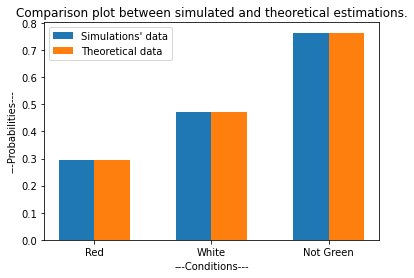
\includegraphics[width=100mm, height=62.4mm]{Assignment 2 graph}

\end{document}
    

